\documentclass[12pt]{beamer}
\usetheme{metropolis}
\definecolor{myblue}{RGB}{34, 70, 135}
\setbeamercolor{frametitle}{fg=white}
\usepackage{listings}
\lstset{
  basicstyle=\ttfamily\small,
  keywordstyle=\color{myblue}\bfseries,
  commentstyle=\color{gray},
  stringstyle=\color{orange},
  showstringspaces=false,
  frame=lines,
  columns=fullflexible,
}
\usepackage{tikz}
\usetikzlibrary{shadows}
\begin{document}
% Stunning Title Slide
{
\begin{frame}[plain]
  \vfill
  \centering
  {\usebeamerfont{title}\usebeamercolor[fg]{title}\Huge \textbf{Kaggle Tweets Classification}\par}
  \vskip1em
  {\usebeamerfont{subtitle}\large Tweets Binary Classification Using ML-DL \LaTeX\par}
  \vskip2em
  {\usebeamerfont{author}\large Nikos Nteits\par}

  \vskip2em
  {\usebeamerfont{date}\normalsize \today\par}
  \vfill


\end{frame}
}
\begin{frame}{Agenda}
  \tableofcontents
\end{frame}

\section{Dataset}

\begin{frame}{Kaggle Tweets Dataset}

\textbf{Each sample in the train and test set has the following information:}
\begin{itemize}
  	\item id - a unique identifier for each tweet.
	 \item text - the text of the tweet.
  	\item location - the location the tweet was sent from (may be blank)
  	\item keyword - a particular keyword from the tweet (may be blank)..
  	\item target - in train.csv only, this denotes whether a tweet is about a real disaster (1) or not (0).
\end{itemize}

\end{frame}


\begin{frame}{Kaggle Tweets Dataset}

\textbf{Relatively Balanced Dataset:}
\begin{itemize}
  	\item target =0 : 4342
	 \item target =0 : 3271

\end{itemize}
\end{frame}

\section{Preprocessing}

\begin{frame}{Preprocessing Steps:}

\begin{itemize}
 \item Special characters Removal
\item Text in square brackets Removal
\item Non-word characters Removal
\item URLs Removal
\item HTML tags Removal
\item Words containing numbers Removal
\item Stopwords Removal
\item Stemming
\end{itemize}
\end{frame}
\section{Processing}
\begin{frame}{Processing:}
\begin{itemize}
\item \textbf{Multiple Vectorization techniques were implemented}
\item \textbf{Multiple models were tried}

\end{itemize}

\end{frame}

\begin{frame}{Vectorizers:}
\begin{itemize}

\item Binary Count Vectorizer
\item Count Vectorizer
\item Tfidf Vectorizer
\item Tfidf Vectorizer 1-2 grams
\item Word2Vec 300 (mean)
\item Glove Twitter 200d
\item USE-4
\item USE-large 5
\item Bertweet base (mean)


\end{itemize}

\end{frame}

\begin{frame}{Models:}
\begin{itemize}
\item Logreg
\item Lasso
\item Ridge
\item SVM
\item Multinomial Naive Bayes
\item Decision Tree


\end{itemize}

\end{frame}

\begin{frame}{Models:}

Combinations of Vectorizers and Models shown above were ran .
At last a Pretrained Roberta Base Model was used with a classification head on top. 
The model was fine tuned for 5 epochs with 0,1 dropout rate and learning rate of 0.00002.
  




\end{frame}

\section{Results}
\begin{frame}{Results:}
\begin{center}
    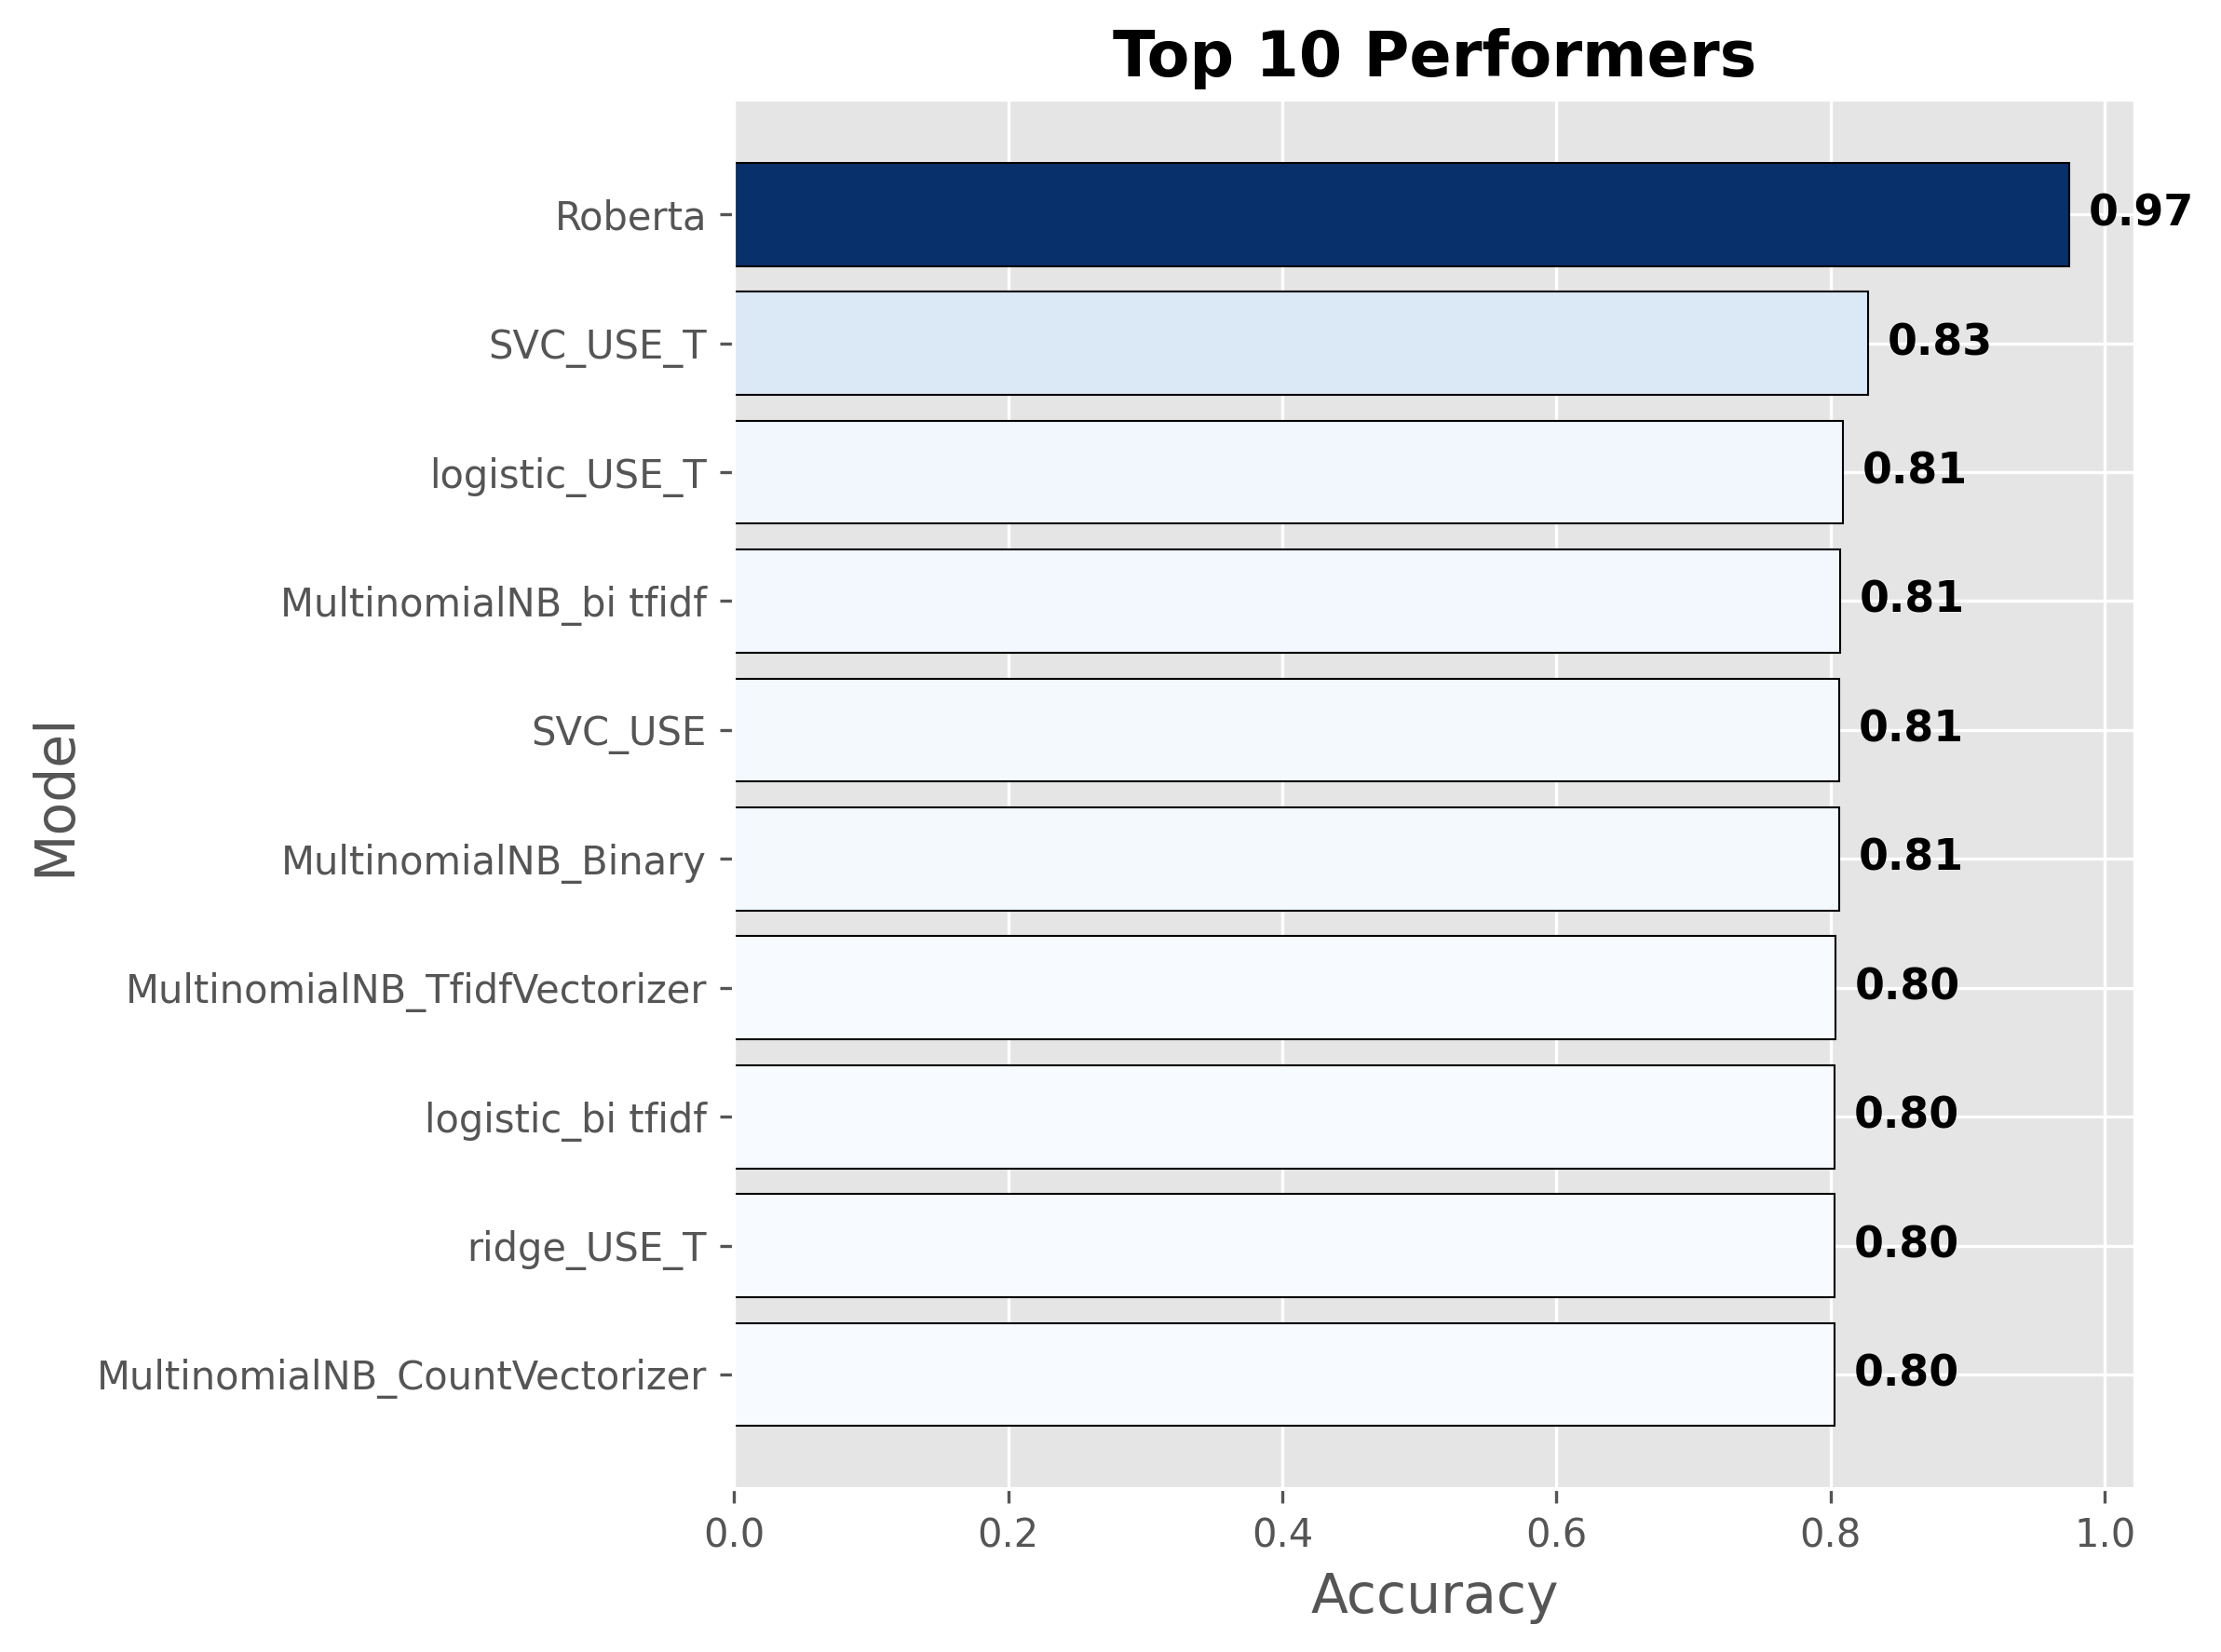
\includegraphics[width=0.7\linewidth]{top10_performers_blue.png}
    
    % Example legend below the image
    \vspace{1em}
    \begin{tabular}{ll}
      \textcolor{black}{ Figure 1 }\\

      % Add more as needed
    \end{tabular}
\end{center}
\end{frame}
\section{Final Remarks}
\begin{frame}{Final Remarks:}

Roberta significantly outperforms every handcrafted Vectorizer-Model combination ,something foreseeable  as the model has been trained on Twitter data hence transfer is natural.As for the rest, universal sentence encoder seems to have an edge over the rest as models with use as vectorizer slightly outperform their coresponding siblings.
  \end{frame}


\end{document}